\documentclass[xcolor=pdftex,dvipsnames,table,mathserif]{beamer}
\usepackage{subfigure}
\usepackage{amsbsy}
\usepackage{tikz}
\usetikzlibrary{arrows}
\usepackage{amsmath,graphicx,dsfont,color}
\usepackage{amsfonts}
\usepackage{amssymb}
\usepackage{array}

\bibliographystyle{apalike}

\setbeamertemplate{bibliography item}{\insertbiblabel}
\setbeamertemplate{bibliography entry title}{}
\setbeamertemplate{bibliography entry location}{}
\setbeamertemplate{bibliography entry note}{}

%Definitiona

\newcommand{\x}{\mathbf{x}}
\newcommand{\X}{\mathbf{X}}
\newcommand{\W}{\mathbf{W}} %Weight
\newcommand{\bais}{\mathbf{b}}%Bais
\newcommand{\act}{\texttt{g}}%Activation
\newcommand{\loss}{L}
\newcommand{\pdata}{\hat{p}_{\texttt{data}}}
\newcommand{\nsize}{n}
\newcommand{\param}{\boldsymbol{\theta}}
\newcommand{\featmap}{\boldsymbol{\phi}}
\newcommand{\EV}{\mathbb{E}}







\usepackage{physics}

\graphicspath{{../graphics/}}

\AtBeginSection[]{
  \begin{frame}{Contents}
  \tableofcontents[currentsection, hideothersubsections]
  \end{frame}
}

\AtBeginSubsection[]{
  \begin{frame}{Contents}
  \tableofcontents[currentsection, subsectionstyle=show/shaded/hide]
  \end{frame}
}

\setbeamertemplate{footline}[frame number]{}
\setbeamertemplate{navigation symbols}{}
\setbeamertemplate{section in toc}[square]
\setbeamertemplate{items}[square]

\title{Fully convolutional neural networks}
\author{E. Decencière}
\date{MINES ParisTech\\
  PSL Research University\\
  Center for Mathematical Morphology
}
\titlegraphic{
\includegraphics[height=1.7cm]{../graphics/logoemp}}

\useinnertheme{rounded}
\usecolortheme{rose}

%%%%%%%%%%%%%%%%%%%%%%%%%%%%%%%%%%%%%%%%%%%%%%%%%%%%%%%
%%%%%%%%%%%%%%%%%%%%%%%%%%%%%%%%%%%%%%%%%%%%%%%%%%%%%%%

\begin{document}

\frame{\titlepage}

\frame{
\frametitle{Contents}
\tableofcontents[hidesubsections]
}

%%%%%%%%%%%%%%%%%%%%%%%%%%%%%%%%%%%%%%%%%%%%%%%%%%
%%%%%%%%%%%%%%%%%%%%%%%%%%%%%%%%%%%%%%%%%%%%%%%%%%
\section{Introduction}

%%%%%%%%%%%%%%%%%%%%%%%%%%%%%%%%%%%%%%%%%%%%%%%%%%
\frame{
  \frametitle{A few words about myself}

  \begin{itemize}

  \item Researcher on mathematical morphology and image processing

  \item Main current application fields:
    \begin{itemize}
    \item Ophthalmology
    \item Dermatology, cosmetology
    \item Astronomy (2 years)
    \end{itemize}
  \item I have been using deep learning methods since 2015

  \end{itemize}

  \begin{block}{Acronyms}
    \begin{itemize}
    \item ANN = artificial neural network
    \item CNN = convolutional neural network
    \end{itemize}
  \end{block}


}


%%%%%%%%%%%%%%%%%%%%%%%%%%%%%%%%%%%%%%%%%%%%%%%%%%
\frame{
\frametitle{Image Segmentation with NNs}

\begin{itemize}

\item Computer vision has been one of the main application domains of NNs

\item Image segmentation often is an important step in an image processing work flow

\item Image segmentation has been a very active deep learning research field

\end{itemize}


\begin{block}{Image segmentation example}
  \begin{figure}
    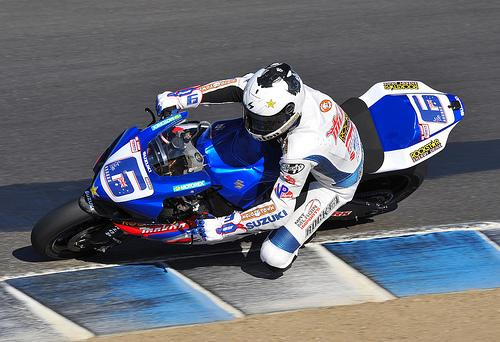
\includegraphics[height=2.5cm]{pascal_moto}
    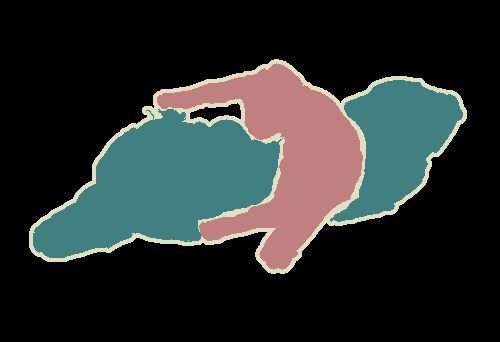
\includegraphics[height=2.5cm]{pascal_moto_seg}
  \end{figure}
\end{block}

}


%%%%%%%%%%%%%%%%%%%%%%%%%%%%%%%%%%%%%%%%%%%%%%%%%%
\frame{
\frametitle{Image definition}

\begin{block}{Definition: image}
  An 2-dimensional image $I$ of size $p \times q$ ($p, q \in \N^*$) is a function from $D = [0, \ldots p-1] \times [0, \ldots q-1]$ into $\R^d$ ($d \in \N^*$).

  The set of these images is $\mathcal{I}^d$.
\end{block}

\begin{block}{Examples}
  \begin{figure}
  \hfill
  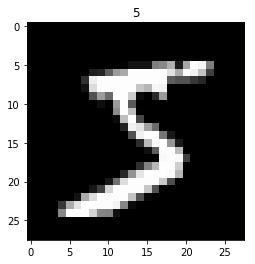
\includegraphics[width=2cm]{mnist_example_5}
  \hfill
  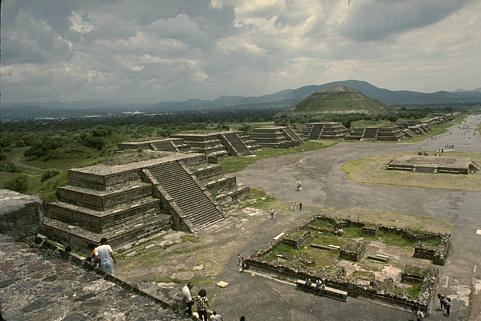
\includegraphics[width=4cm]{berkeley_db_33066.jpg}
  \caption{$28 \times 28$ grey level image $(d=1)$ from the MNIST dataset, and $481 \times 321$ colour image $(d=3)$ from the Berkeley segmentation dataset.}
\end{figure}
\end{block}


}


%%%%%%%%%%%%%%%%%%%%%%%%%%%%%%%%%%%%%%%%%%%%%%%%%%
\frame{
\frametitle{Image-to-image NN}

\begin{block}{Definition: image-to-image neural network}
  An image-to-image NNs $F$ is a NN that transforms an image into an image of same size:
  \vspace{-1em}
  \begin{align*}
    F: \,& \mathcal{I}^{d_1} \longrightarrow \mathcal{I}^{d_2} \\
    & I               \longmapsto     N(I)
  \end{align*}
  Note that the dimensions $d_1$ and $d_2$ of the value spaces can be different.
\end{block}

}


%%%%%%%%%%%%%%%%%%%%%%%%%%%%%%%%%%%%%%%%%%%%%%%%%%
\frame{
\frametitle{Examples}

\begin{block}{Bulge / disk decomposition}
  \begin{figure}
    %% \includegraphics[width=2cm]{galaxy.png}
    %% $\longrightarrow$
    %% \includegraphics[width=2cm]{disk.png}
    %% $+$
    %% \includegraphics[width=2cm]{bulge.png}
    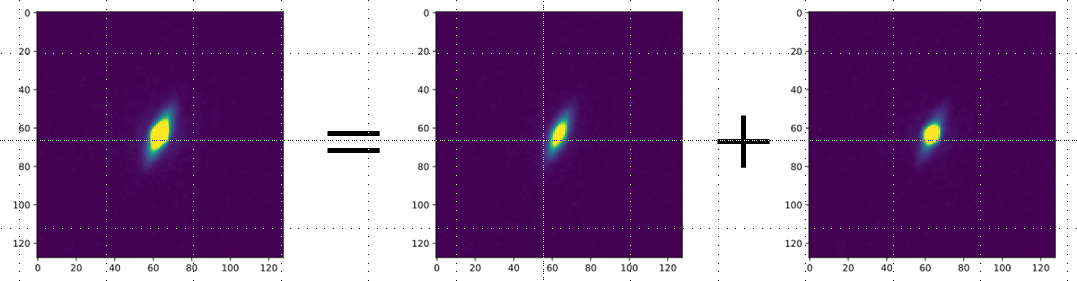
\includegraphics[width=8cm]{decomposition.png}\\
    \hfill {\tiny (Credits: Tuccillo, Huertas-Company, Velasco-Forero, Decencière)}
\end{figure}
\end{block}

\pause

\begin{block}{Deblurring network \cite{hradis_convolutional_2015}}
  \begin{figure}
  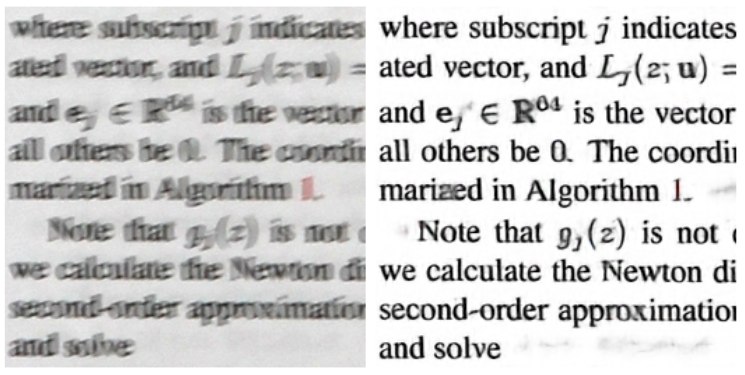
\includegraphics[width=4cm]{deblurring_hradis.png}
\end{figure}
\end{block}


}

%%%%%%%%%%%%%%%%%%%%%%%%%%%%%%%%%%%%%%%%%%%%%%%%%%
\frame{
\frametitle{Image-to-image NNs architecture}

\begin{itemize}

\item Image-to-image NNs are based on convolutional layers

\item If downsampling is used, the corresponding upsampling is needed

\item The \alert{receptive field} of the network is an essential property

\end{itemize}

\pause

\begin{block}{Example: Pang network \cite{pang_cell_2010}}
  \begin{figure}
    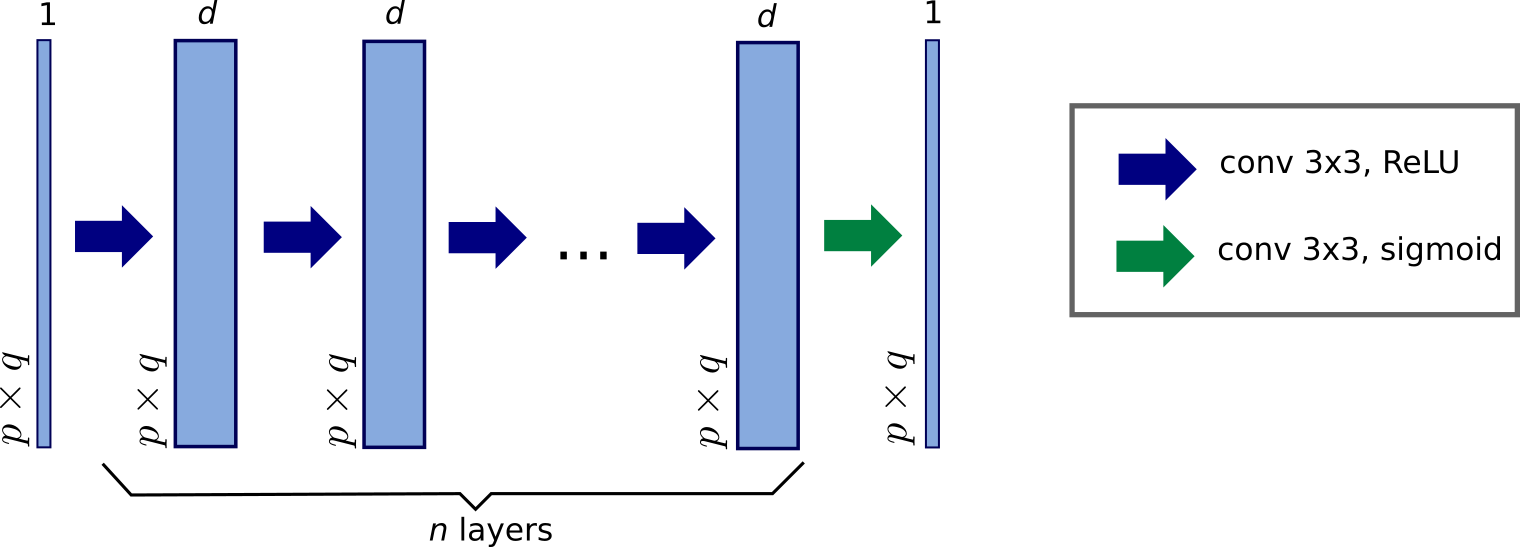
\includegraphics[width=6cm]{plain_convnet.png}
  \end{figure}
\end{block}

}

%%%%%%%%%%%%%%%%%%%%%%%%%%%%%%%%%%%%%%%%%%%%%%%%%%
\frame{
\frametitle{Receptive field}

\begin{block}{Definition: links between neurons}
  In a NN, we say that neuron $a$ is linked to neuron $b$ if there is an oriented path in the corresponding graph going from $a$ to $b$.
\end{block}


\begin{block}{Definition}
  The \alert{receptive field} of a neuron in a NN is the set of input neurons that are linked to that neuron.

  The size of the receptive field is an essential property when designing a fully-convolutional NN architecture.
\end{block}

}


%%%%%%%%%%%%%%%%%%%%%%%%%%%%%%%%%%%%%%%%%%%%%%%%%%
\frame{
\frametitle{Receptive field of the Pang network}

\begin{block}{What is the size of the receptive field of the neurons in the last layer?}
  \begin{figure}
    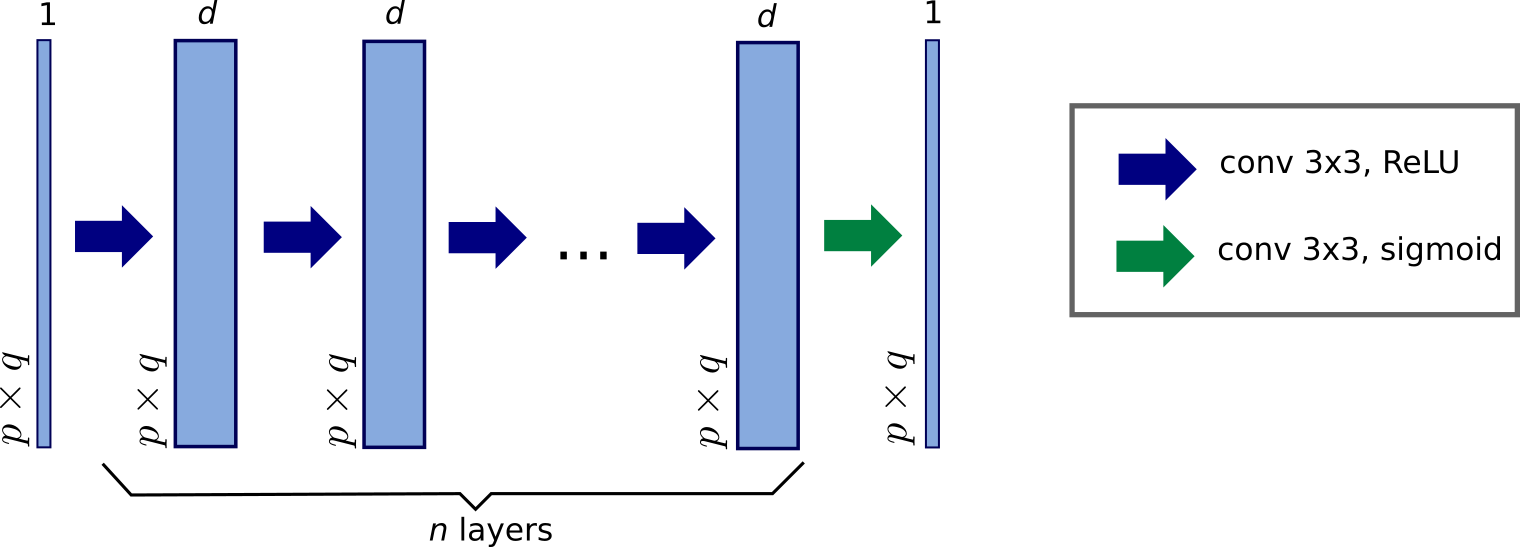
\includegraphics[width=6cm]{plain_convnet.png}
  \end{figure}
\end{block}

\vspace{1em}

\pause

\centering
Answer: $1 + 2 \times (n+1)$

}
%%%%%%%%%%%%%%%%%%%%%%%%%%%%%%%%%%%%%%%%%%%%%%%%%%
\frame{
\frametitle{The specific case of image segmentation}

\begin{block}{Definition: image segmentation}
  Let $I$ be an image defined on $D$. A segmentation of $I$ is a partition of $D$. In practice the regions of the segmentation should correspond to the objects in $I$, which is application dependant.
\end{block}


\begin{itemize}

\item A partition is often represented as a labelled image

\item In order to make the segments symmetric, each one is represented by a different channel

\end{itemize}

}



%%%%%%%%%%%%%%%%%%%%%%%%%%%%%%%%%%%%%%%%%%%%%%%%%%
\frame{
\frametitle{Some vocabulary on segmentation}

\begin{itemize}

\item \textbf{Object detection / localization}: bounding box around the object(s).
\item \textbf{Binary segmentation}: segmentation in 2 classes, background and object.
\item \textbf{Semantic segmentation}: a label is given to each pixel, according to the object it belongs to.
\item \textbf{Instance segmentation}: identify each separate object, even if they belong to the same class.

\end{itemize}

}
%%%%%%%%%%%%%%%%%%%%%%%%%%%%%%%%%%%%%%%%%%%%%%%%%%
%%%%%%%%%%%%%%%%%%%%%%%%%%%%%%%%%%%%%%%%%%%%%%%%%%
\section{Binary segmentation}

%%%%%%%%%%%%%%%%%%%%%%%%%%%%%%%%%%%%%%%%%%%%%%%%%%%%%
\frame{
  \frametitle{Neuron membrane segmentation challenge (ISBI 2012)}

  \begin{itemize}
  \item Train: single stack of size $30\times512\times512$.
  \item Test: a second stack of same size.
  \end{itemize}

  \begin{figure}
    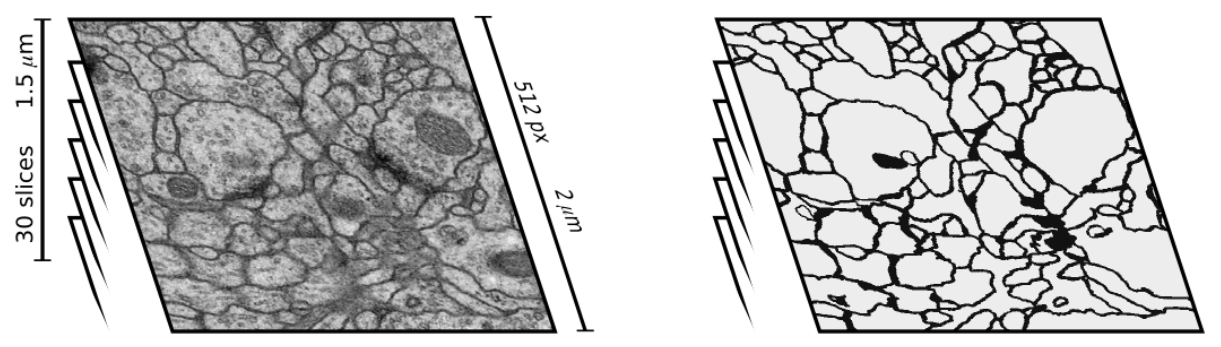
\includegraphics[width=9cm]{em_challenge}
  \end{figure}

}

%%%%%%%%%%%%%%%%%%%%%%%%%%%%%%%%%%%%%%%%%%%%%%%%%%%%%
\frame{
  \frametitle{Neuron membrane segmentation challenge winner~\cite{ciresan_deep_2012}}

  \begin{figure}
    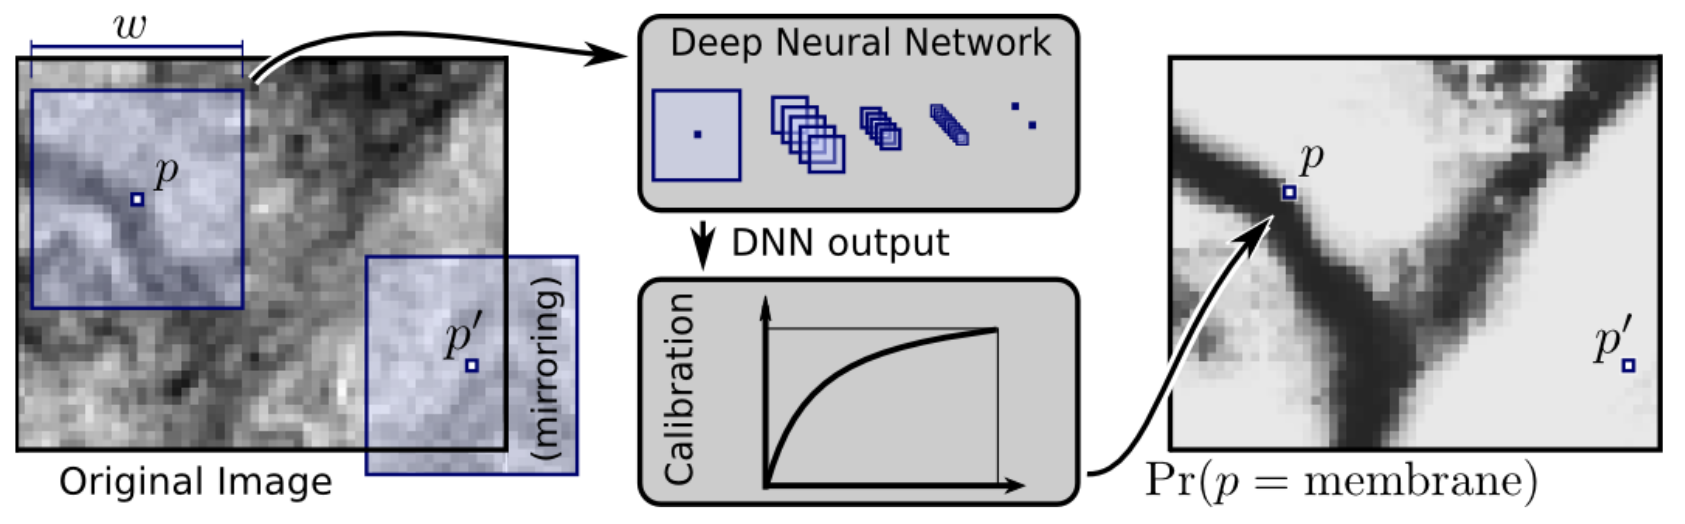
\includegraphics[width=9cm]{dnn_ciresan}
  \end{figure}

}

%%%%%%%%%%%%%%%%%%%%%%%%%%%%%%%%%%%%%%%%%%%%%%%%%%
%%%%%%%%%%%%%%%%%%%%%%%%%%%%%%%%%%%%%%%%%%%%%%%%%%
\section{Semantic segmentation}


%%%%%%%%%%%%%%%%%%%%%%%%%%%%%%%%%%%%%%%%%%%%%%%%%%%%%
\frame{
  \frametitle{Pascal visual object classes segmentation challenge 2012 \cite{everingham_pascal_2014}}

  \begin{itemize}
  \item 1464 training and 1449 validation images
  \item automatic online test, with unknown images
  \item 20 image categories (cat, sofa, motorbike, person, etc.)
  \end{itemize}

  \begin{figure}
    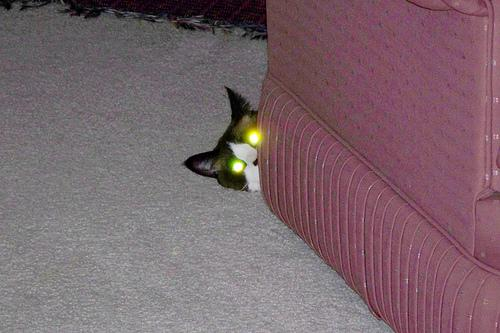
\includegraphics[height=2.5cm]{pascal_cat}
    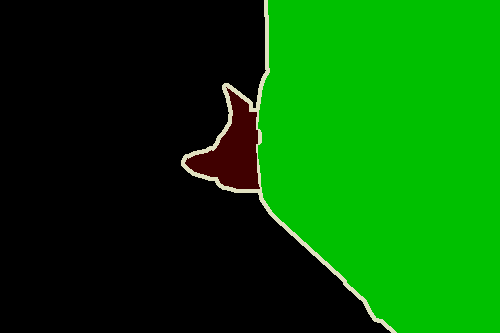
\includegraphics[height=2.5cm]{pascal_cat_seg}\\
    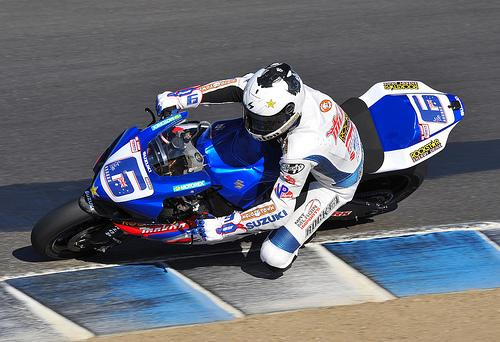
\includegraphics[height=2.5cm]{pascal_moto}
    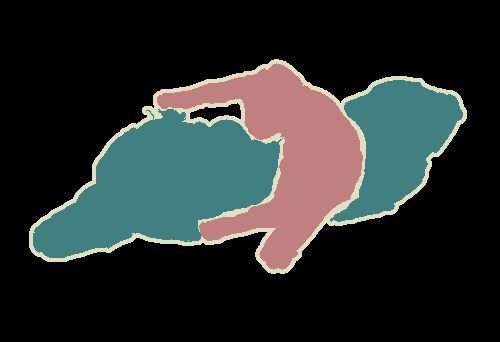
\includegraphics[height=2.5cm]{pascal_moto_seg}
  \end{figure}

}

%%%%%%%%%%%%%%%%%%%%%%%%%%%%%%%%%%%%%%%%%%%%%%%%%%%%%

\frame{
  \frametitle{Convolutional nets for semantic image segmentation}

  Three papers in 2015:

  \begin{itemize}

  \item Fully convolutional networks for semantic segmentation \cite{long_fully_2015}
  \item U-Net: convolutional networks for biomedical image segmentation \cite{ronneberger_u-net:_2015}
  \item SegNet: A Deep Convolutional Encoder-Decoder Architecture for Image Segmentation \cite{badrinarayanan_segnet:_2015}

  \end{itemize}


}

%%%%%%%%%%%%%%%%%%%%%%%%%%%%%%%%%%%%%%%%%%%%%%%%%%

\frame{
\frametitle{Example: U-Net architecture \cite{ronneberger_u-net:_2015}}

\begin{figure}
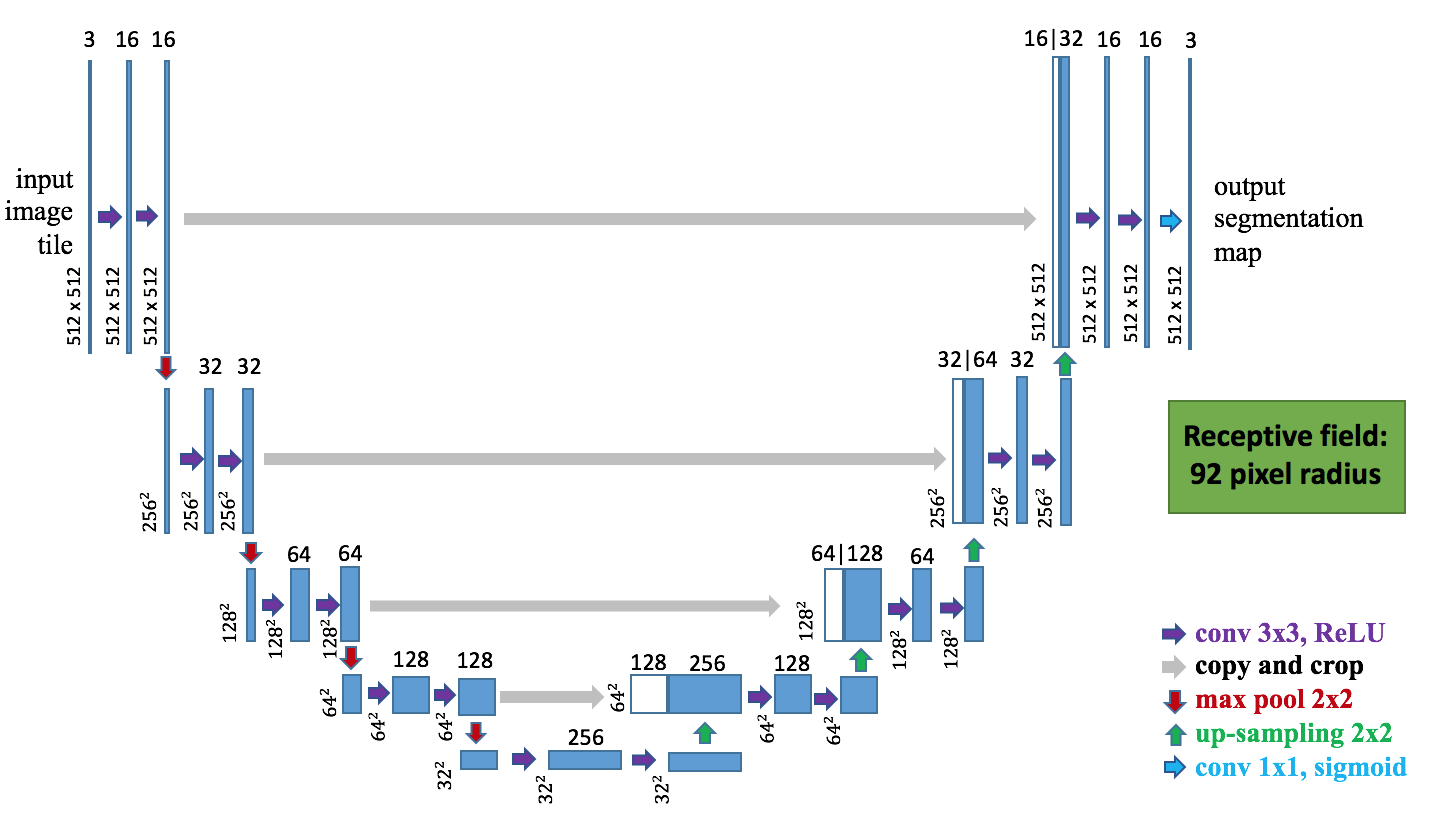
\includegraphics[height=6cm]{unet}
\end{figure}
}

%%%%%%%%%%%%%%%%%%%%%%%%%%%%%%%%%%%%%%%%%%%%%%%%%%

\frame{
\frametitle{What is the size of the receptive field of U-Net}


\begin{figure}
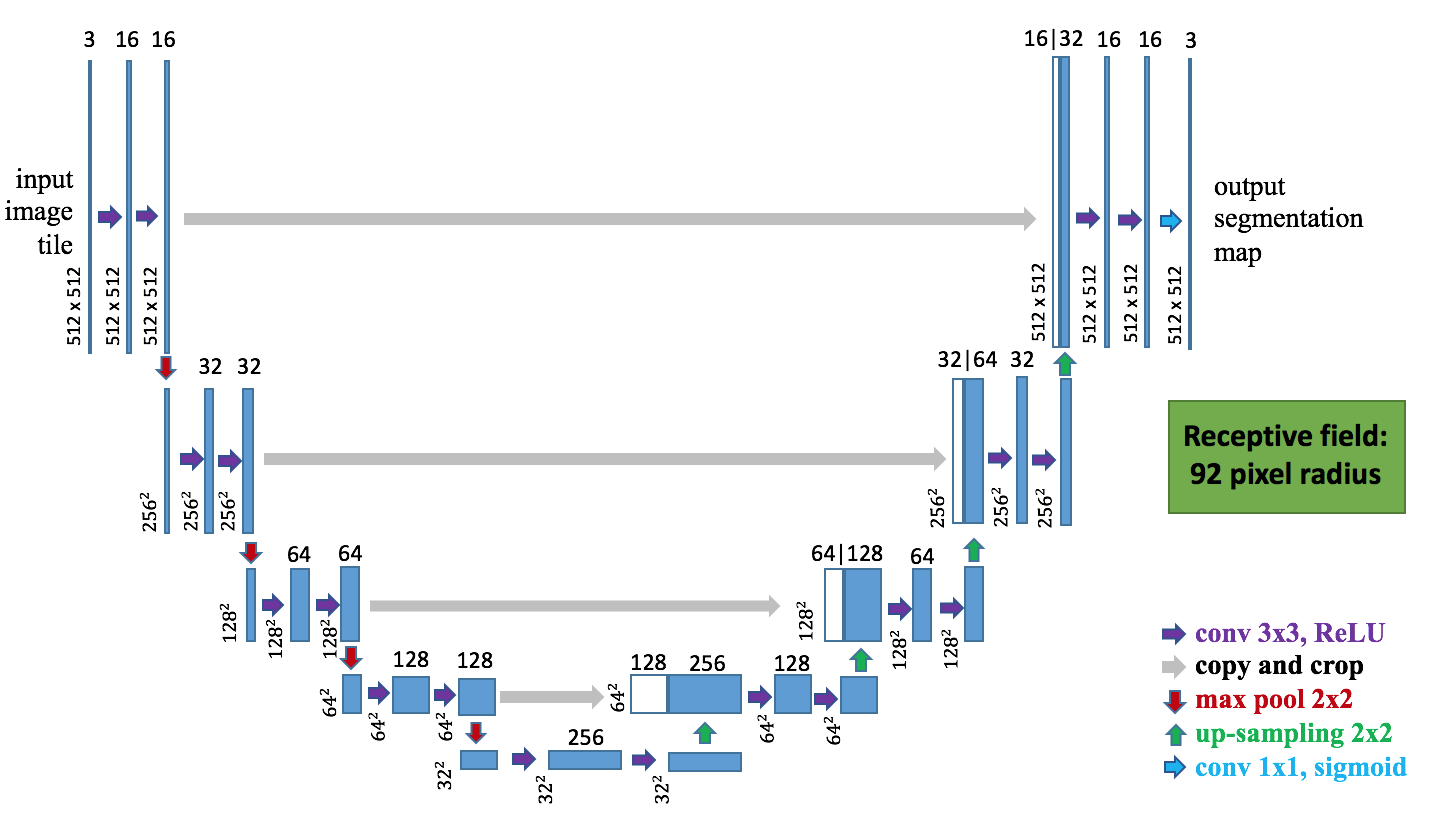
\includegraphics[height=5cm]{unet}
\end{figure}


\pause

  \centering
  Answer: $185 \times 185$
}

%%%%%%%%%%%%%%%%%%%%%%%%%%%%%%%%%%%%%%%%%%%%%%%%%%

\frame{
\frametitle{Example: SegNet architecture \cite{badrinarayanan_segnet:_2015}}

\begin{figure}
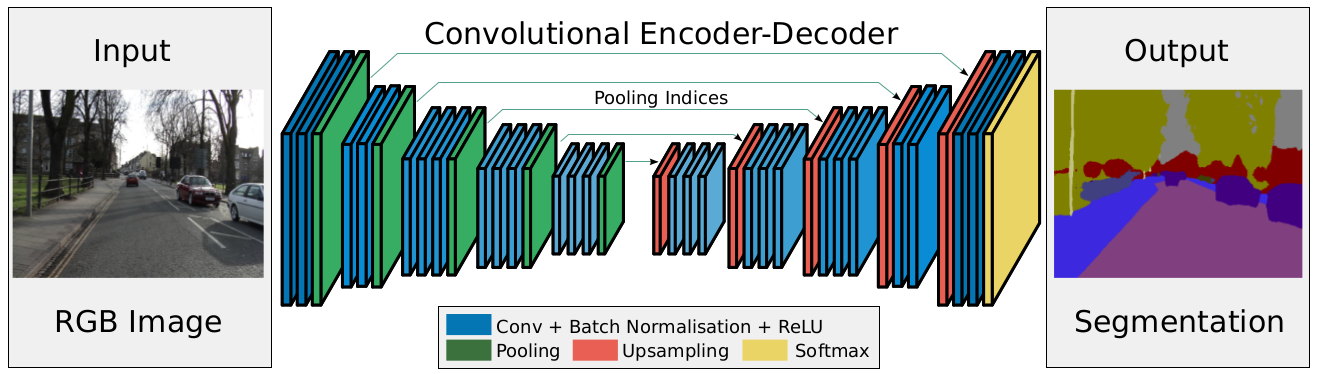
\includegraphics[width=9cm]{segnet_archi}
\end{figure}
}

%%%%%%%%%%%%%%%%%%%%%%%%%%%%%%%%%%%%%%%%%%%%%%%%%%

\frame{
  \frametitle{Remarks}

  \begin{itemize}
  \item These architectures easily contain a number of parameters of the order of $10^7$ (28 million for U-Net)
  \item Their optimization might be difficult
  \item For many segmentation applications, they are overkill
    \begin{itemize}
    \item But you can reduce the number of filters or the number of layers
      \end{itemize}
  \end{itemize}

  }

%%%%%%%%%%%%%%%%%%%%%%%%%%%%%%%%%%%%%%%%%%%%%%%%%%%%%
%%%%%%%%%%%%%%%%%%%%%%%%%%%%%%%%%%%%%%%%%%%%%%%%%%%%%
\section{Instance segmentation}
%%%%%%%%%%%%%%%%%%%%%%%%%%%%%%%%%%%%%%%%%%%%%%%%%%

\frame{
  \frametitle{COCO: common objects in context \cite{lin_microsoft_2014}}

\begin{itemize}
  \item $2$ million objects, from $80$ categories, in $300\,000$ images
\end{itemize}


\begin{figure}
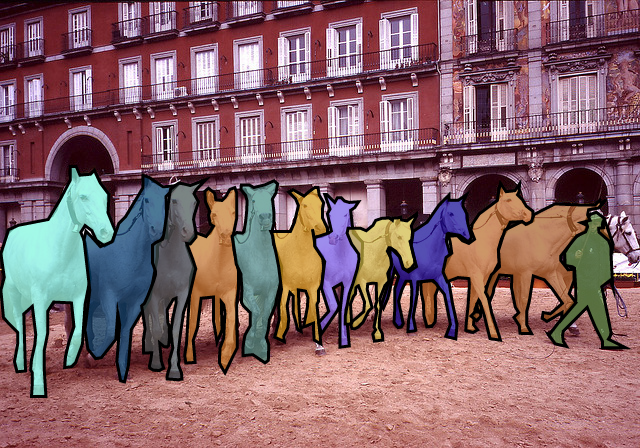
\includegraphics[height=3.4cm]{coco_ex_horses}
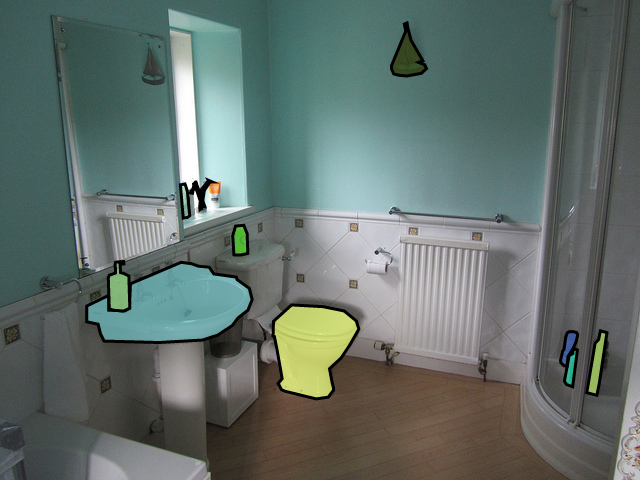
\includegraphics[height=3.4cm]{coco_ex_salle_de_bain}
\end{figure}

\begin{block}{}
Winner 2016: Fully Convolutional Instance-aware Semantic Segmentation (Microsoft) \cite{li_fully_2016}
  \end{block}

}


%%%%%%%%%%%%%%%%%%%%%%%%%%%%%%%%%%%%%%%%%%%%%%%%%%%%%
\frame{
\frametitle{COCO instance segmentation challenge: examples of 2016 winner results}

\begin{figure}
  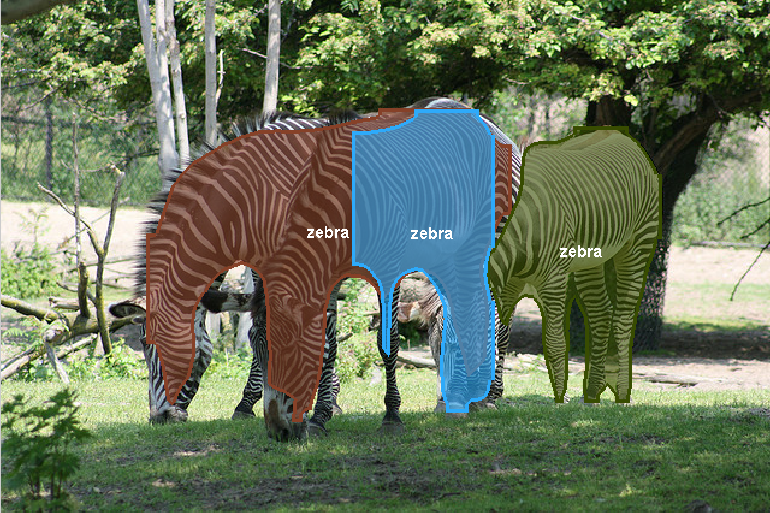
\includegraphics[width=4.5cm]{COCO_test2015_000000003241.png}
  \hspace{1cm}
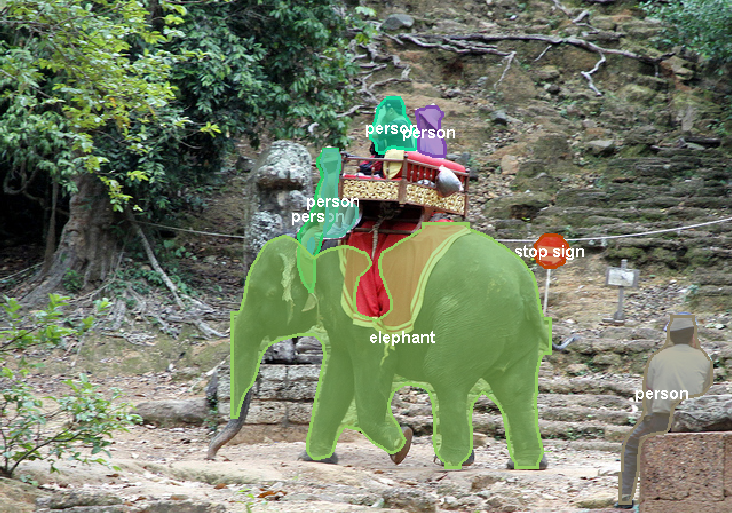
\includegraphics[width=4.5cm]{COCO_test2015_000000004178.png}\\
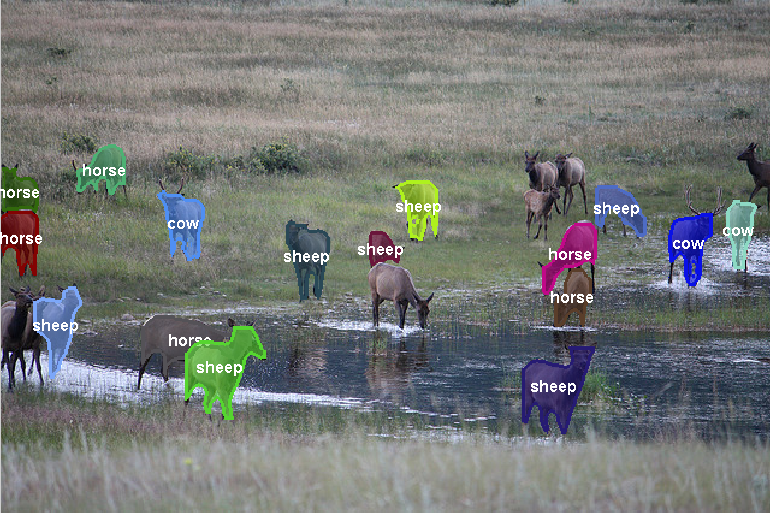
\includegraphics[width=4.5cm]{COCO_test2015_000000006147.png}
\hspace{1cm}
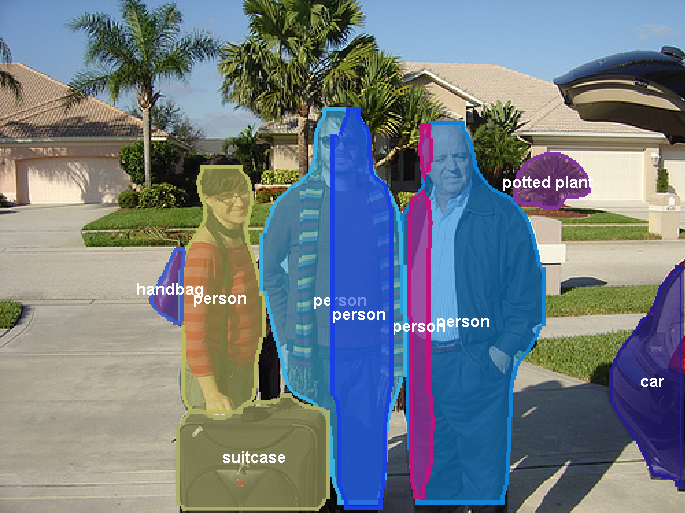
\includegraphics[width=4.5cm]{COCO_test2015_000000016177.png}
\end{figure}

}

%%%%%%%%%%%%%%%%%%%%%%%%%%%%%%%%%%%%%%%%%%%%%%%%%%%%%
\frame{
  \frametitle{State of the art on the COCO database: Mask R-CNN \cite{he_mask_2017}}

  \begin{figure}
    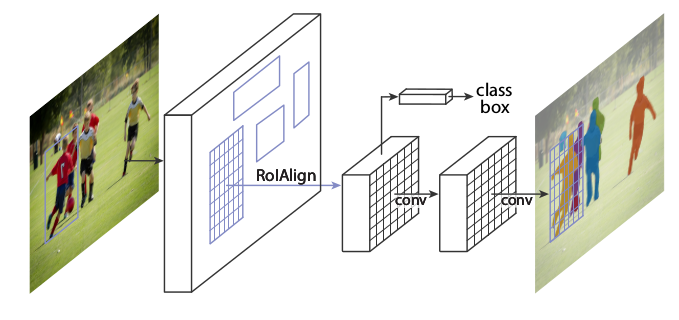
\includegraphics[width=7.5cm]{mask_r_cnn.png}
  \end{figure}
}

%%%%%%%%%%%%%%%%%%%%%%%%%%%%%%%%%%%%%%%%%%%%%%%%%%%%%
\frame{
  \frametitle{Mask R-CNN on the COCO database}

  \begin{figure}
    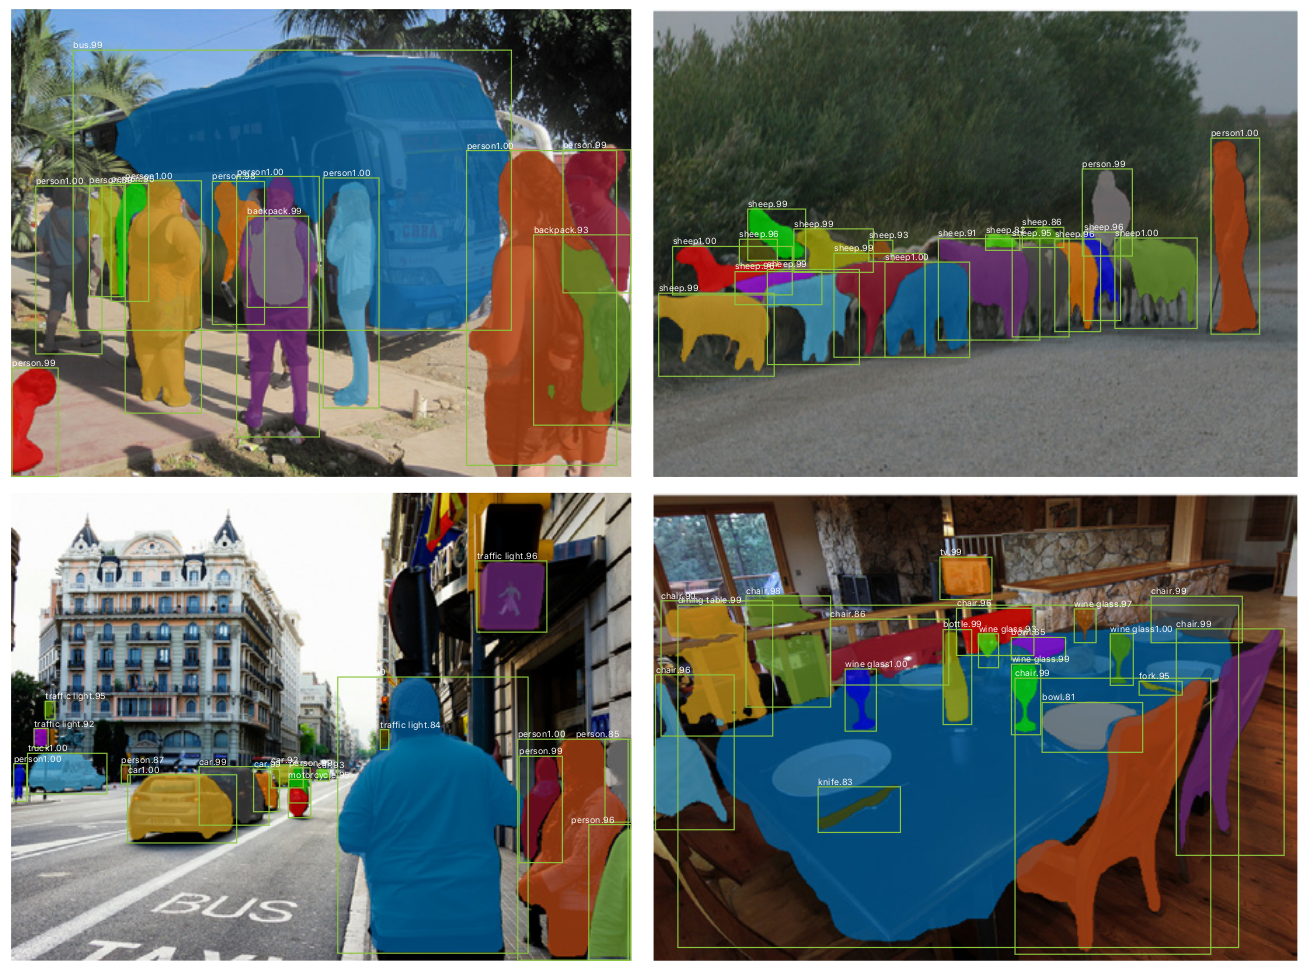
\includegraphics[width=9cm]{mask_r_cnn_examples.png}
  \end{figure}

  }

%%%%%%%%%%%%%%%%%%%%%%%%%%%%%%%%%%%%%%%%%%%%%%%%%%%%%
\frame{
  \frametitle{Partially supervised segmentation - \cite{hu_learning_2017}}

  \begin{itemize}
    \item 80 segmented categories from COCO database
    \item 3000 visual concepts using box annotations from the Visual Genome dataset (100k images)
    \end{itemize}

  \begin{figure}
    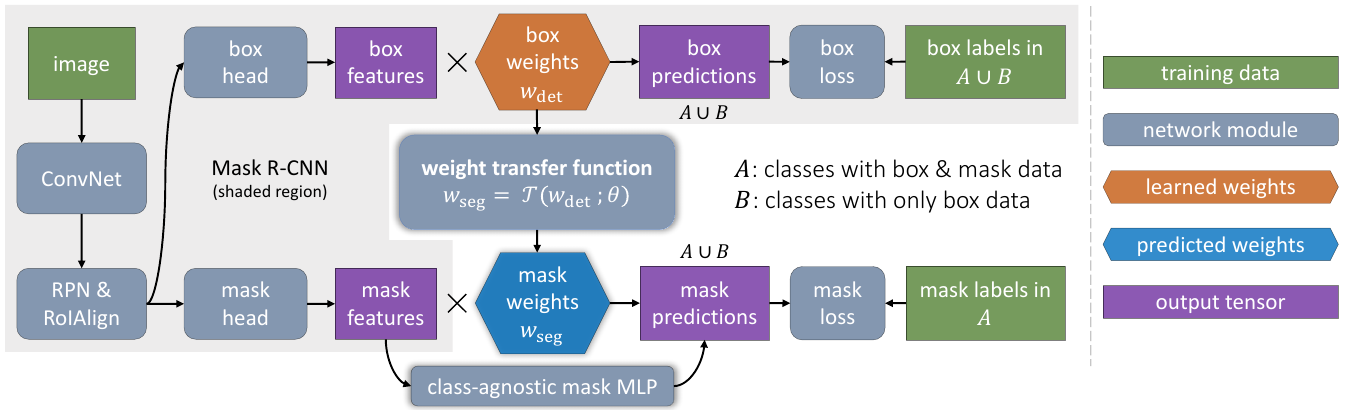
\includegraphics[width=12cm]{segm_every_thing_method.png}
  \end{figure}

  }

%%%%%%%%%%%%%%%%%%%%%%%%%%%%%%%%%%%%%%%%%%%%%%%%%%%%%
\frame{
  \frametitle{Partially supervised segmentation - learning to segment every thing}

  \begin{figure}
    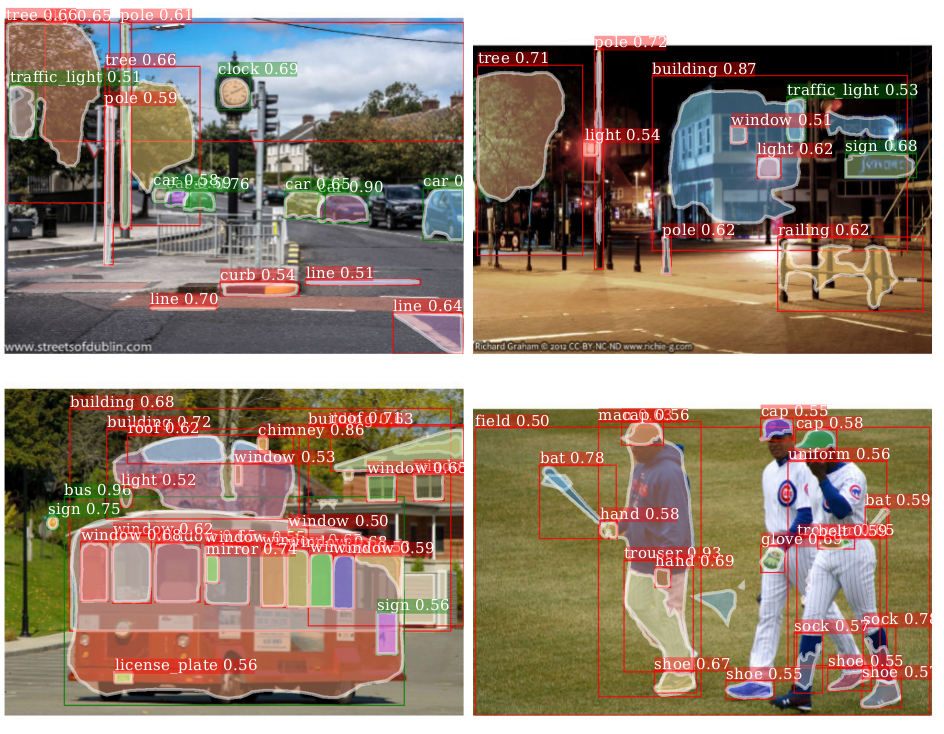
\includegraphics[width=8cm]{segment_every_thing.png}
  \end{figure}

\cite{hu_learning_2017}

  }

%%%%%%%%%%%%%%%%%%%%%%%%%%%%%%%%%%%%%%%%%%%%%%%%%%
\frame{
  \frametitle{Current (?) trends for instance segmentation}

  \begin{itemize}

  \item Region proposal +
  \item Fully convolutional (very deep) network +
  \item (Post-processing)

  \end{itemize}

  \begin{figure}
    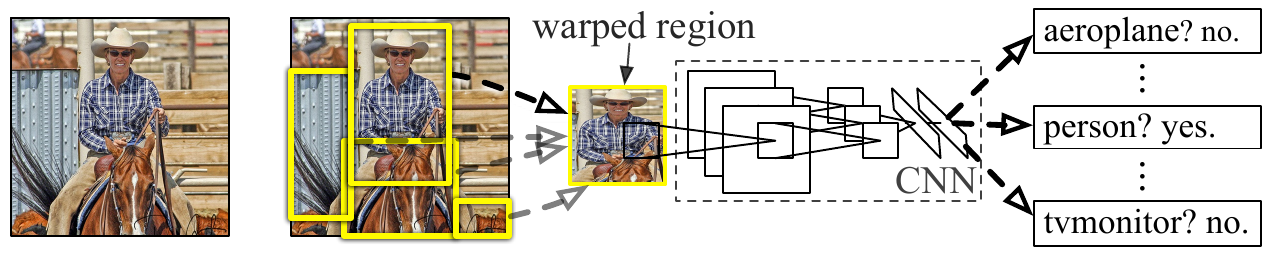
\includegraphics[width=9.5cm]{r_cnn.png}
    \caption{Regions with CNN features (R-CNN) (from \cite{girshick_rich_2014})}
  \end{figure}

  \begin{block}<2->{Meanwhile, on the object detection field...}
  \begin{itemize}
    \item YOLO: you look only once \cite{redmon_yolo9000:_2016}
    \item SSD: single shot detector \cite{liu_ssd:_2016}
  \end{itemize}
  \end{block}

}

%%%%%%%%%%%%%%%%%%%%%%%%%%%%%%%%%%%%%%%%%%%%%%%%%%

%% \frame{
%% \frametitle{A typical convolutional architecture for image classification}

%% \begin{figure}
%%   \includegraphics[width=9.5cm]{conv_net_classif}
%%   \caption{Architecture used for the classification of the NORB dataset (from \cite{scherer_evaluation_2010})}
%% \end{figure}

%% Note that layer P4 can be seen as made of features, which are then classified by the two fully connected layers.


%% }

%%%%%%%%%%%%%%%%%%%%%%%%%%%%%%%%%%%%%%%%%%%%%%%%%%
\section{Practical recommendations}

%%%%%%%%%%%%%%%%%%%%%%%%%%%%%%%%%%%%%%%%%%%%%%%%%%%%%
\frame{
  \frametitle{Modeling your problem}

  \begin{block}{Casting your problem into the right representation}
    \begin {itemize}
    \item Familiarize yourself with the training data (input and output images)
    \item Choose the right representation for your images
    \item Choose an architecture and train it
    \item Analyze the results on the validation data (\alert{look} at the images!)
    \item Do you need preprocessing? Data augmentation? Post-processing?
    \item Iterate ...
    \item Only at the end: test!
    \end{itemize}

  \end{block}

}

%%%%%%%%%%%%%%%%%%%%%%%%%%%%%%%%%%%%%%%%%%%%%%%%%%%%%
\frame{
  \frametitle{Preprocessing}

  \begin {itemize}
  \item Standard statistical preprocessing: not always useful, and sometimes problematic, when applied to images
    \item Morphological operators
  \end{itemize}

}


%%%%%%%%%%%%%%%%%%%%%%%%%%%%%%%%%%%%%%%%%%%%%%%%%%%%%
\frame{
  \frametitle{Data augmentation}

  \begin {itemize}
\item Geometrical transformations: similarities
\item Elastic transformations
\item Specific methods: articulated objects, \ldots
\item Simulated data
  \end{itemize}

}


%%%%%%%%%%%%%%%%%%%%%%%%%%%%%%%%%%%%%%%%%%%%%%%%%%%%%
\frame{
  \frametitle{Postprocessing for segmentation}

  \begin {itemize}
\item Superpixels (e.g. \cite{farabet_learning_2013})
\item Conditional random fields (e.g. \cite{krahenbuhl_efficient_2011})
\item Mathematical morphology
  \end{itemize}

}

%%%%%%%%%%%%%%%%%%%%%%%%%%%%%%%%%%%%%%%%%%%%%%%%%%%%%
\frame{
  \frametitle{What loss to use?}

  \begin{itemize}
  \item Classical choice: mean squared error or cross-entropy
  \item My recommendation: Dice or Jaccard losses
  \end{itemize}

}

%%%%%%%%%%%%%%%%%%%%%%%%%%%%%%%%%%%%%%%%%%%%%%%%%%%%%
\begin{frame}{Practical example}
    \begin{columns}[c]
    \column{.5\textwidth}
        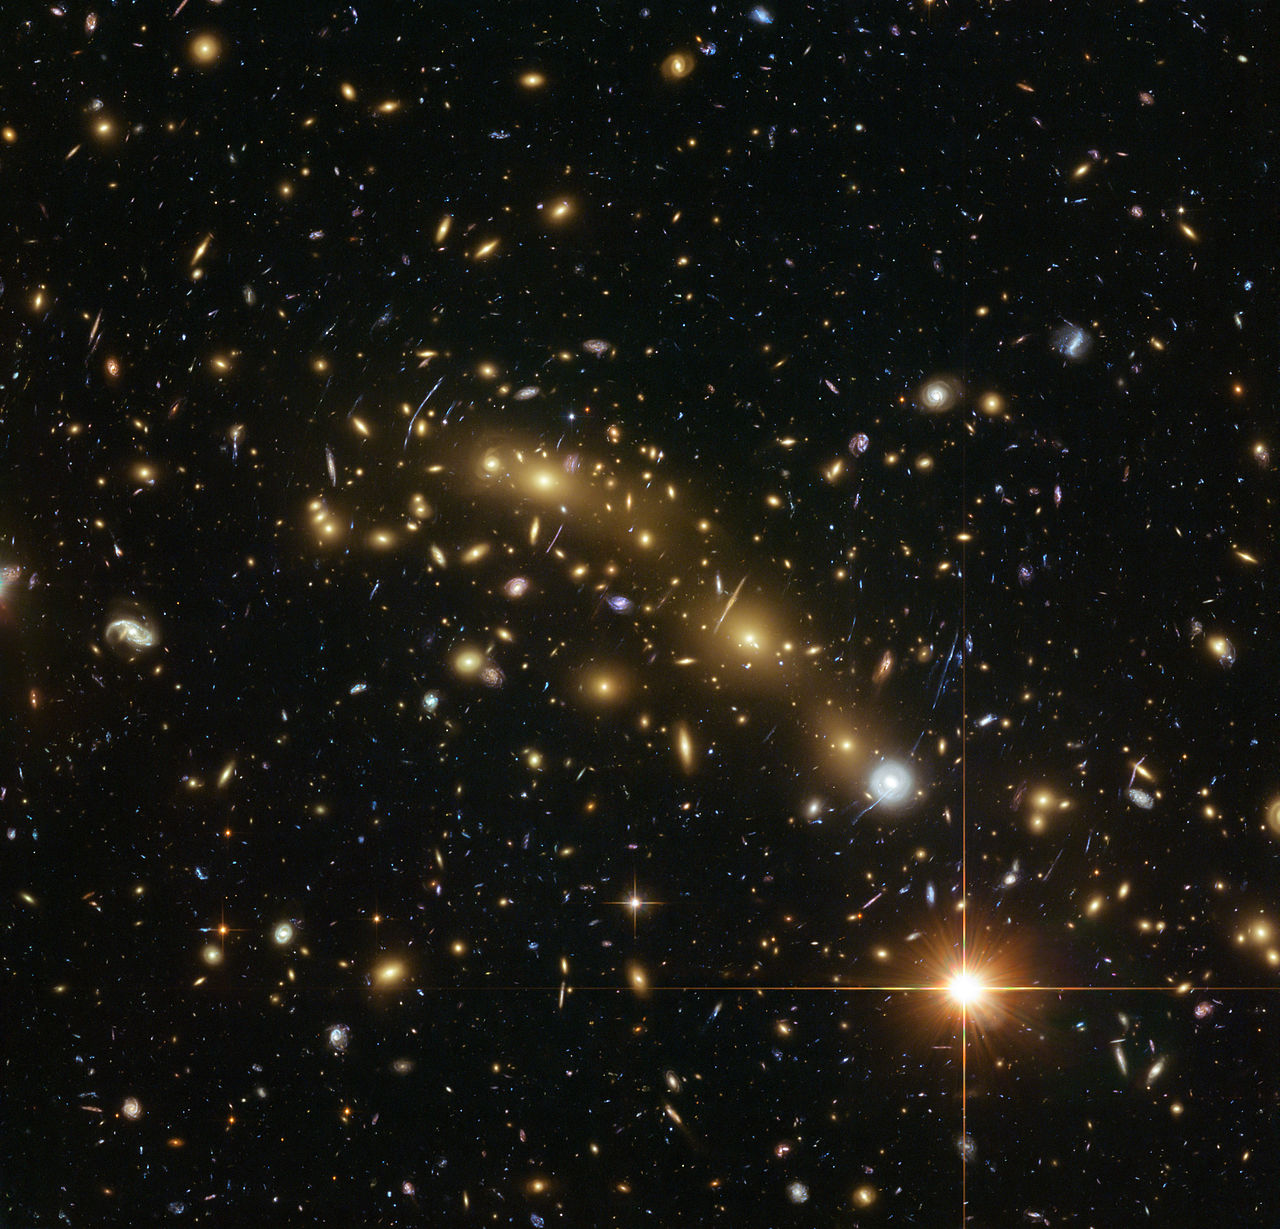
\includegraphics[width=0.9\textwidth]{hst.jpg}\\
        {\tiny (Credits: ESA/Hubble, CC BY 4.0, https://commons.wikimedia.org/w/index.php?curid=34205833)}
    \column{.5\textwidth}
      How would you:
      \begin{itemize}
      \item segment the background?
      \item segment the sources?
      \item separate the sources?
      \end{itemize}

    \end{columns}
\end{frame}


%%%%%%%%%%%%%%%%%%%%%%%%%%%%%%%%%%%%%%%%%%%%%%%%%%%%%
\frame{
  \frametitle{What precision is needed for the ground-truth?}

  \begin{itemize}
  \item The ground truth boundaries do not need to be very precise
  \item
  \end{itemize}

}

%%%%%%%%%%%%%%%%%%%%%%%%%%%%%%%%%%%%%%%%%%%%%%%%%%%%%
\frame{
  \frametitle{Using a CNN}

  \begin{itemize}
  \item A fully convolutional neural network is translation invariant
  \item Provided that the image size is compatible with network's subsampling process, in theory any image can be processed
  \item Practical limit: the memory of the system
  \end{itemize}

}



%%%%%%%%%%%%%%%%%%%%%%%%%%%%%%%%%%%%%%%%%%%%%%%%%%
%%%%%%%%%%%%%%%%%%%%%%%%%%%%%%%%%%%%%%%%%%%%%%%%%%
\section{Conclusion}

%%%%%%%%%%%%%%%%%%%%%%%%%%%%%%%%%%%%%%%%%%%%%%%%%%%%%
\frame{
  \frametitle{A solved problem?}

  \begin {itemize}
  \item Progress in image segmentation during the 5 last years has been enourmous
  \item Several complex problems have now satisfactory solutions
  \item Training can be a problem (large annotated databases, difficult optimization)
  \item Some remaining challenges:
    \begin{itemize}
      \item Making the training database as small as possible
      \item Taking  {\it a priori} structural information into account
      \end{itemize}
   \end{itemize}

  }

%%%%%%%%%%%%%%%%%%%%%%%%%%%%%%%%%%%%%%%%%%%%%%%%%%%%%
%% \frame{
%%   \frametitle{Application to the segmentation of retinal structures}

%%   \begin {itemize}
%%   \item Do we have enough annotated data?
%%   \item Sliding window or global approach?
%%   \item Is our problem translation invariant?
%%   \end{itemize}

%% }

%%%%%%%%%%%%%%%%%%%%%%%%%%%%%%%%%%%%%%%%%%%%%%%%%%

%%%%%%%%%%%%%%%%%%%%%%%%%%%%%%%%%%%%%%%%%%%%%%%%%%
\section*{References}

%%%%%%%%%%%%%%%%%%%%%%%%%%%%%%%%%%%%%%%%%%%%%%%%%%

\frame[allowframebreaks]{

\scriptsize

\frametitle{References}

%\bibliographystyle{amsalpha}
%\bibliographystyle{apalike}

\bibliography{edf.bib}

\normalsize

}




\end{document}
